% \documentclass[sigconf,nonacm]{acmart}
\documentclass[manuscript,screen,nonacm]{acmart}

\usepackage{enumitem}
\setlist[enumerate,1]{label=\arabic*.}
\usepackage{siunitx}
\usepackage{hyperref}
\usepackage{cleveref}
\usepackage{graphicx}
\usepackage{tabularx}
\usepackage{float}
\usepackage[table]{xcolor}
\usepackage{tikz}
\usetikzlibrary{automata,positioning,arrows.meta}
\usepackage{bytefield}

\newcommand{\mypara}[1]{\smallskip\noindent\textbf{#1.}}

\AtBeginDocument{%
  \providecommand\BibTeX{{%
    Bib\TeX}}}

\settopmatter{printfolios=true}

\begin{document}

\title{Resilient Decentralized Communication for Grassroots Social Networks using BLE}

\maketitle

%%%%%%%%%%%%%%%%%%%%%%%%%%%%%%%%%%%%%%%%%%%%%%%%%%%%%%%%%%%%%%%%%%%%%%%%%%%%%%%
\section{Introduction}
%%%%%%%%%%%%%%%%%%%%%%%%%%%%%%%%%%%%%%%%%%%%%%%%%%%%%%%%%%%%%%%%%%%%%%%%%%%%%%%

We assume people with smartphones, each equipped with a permanent keypair, unique with high probability. Public keys are public and never rotated.

We assume a social graph (SG), in which people know the public key of their friends and their friends of friends. Furthermore, we assume that people use the last 128 bits of their public key as their BLE Service UUID. Thus, a person can compute the Service UUID of their friends and friends of friends. Smartphones alternate between advertising and scanning.

We are interested in two scenarios:
\begin{enumerate}
    \item \textbf{Given SG:} Can people find their friends and friends of friends and establish connections, for the purpose of direct communication as well as forwarding?
    \item \textbf{Growing SG:} Can a person perform a ``cold call'' and introduce themselves to another person that is advertising, and establish a connection?
\end{enumerate}

%%%%%%%%%%%%%%%%%%%%%%%%%%%%%%%%%%%%%%%%%%%%%%%%%%%%%%%%%%%%%%%%%%%%%%%%%%%%%%%
\section{Goals}
%%%%%%%%%%%%%%%%%%%%%%%%%%%%%%%%%%%%%%%%%%%%%%%%%%%%%%%%%%%%%%%%%%%%%%%%%%%%%%%

\begin{enumerate}
  \item Enable communication in first-contact between complete strangers $U,V$ (no common friends of degree $\le 2$), pending mutual consent
  \item Enable communication in first-contact between $n$-degree friends $U,V$ ($n \le 2$): $U$ has common friends with $V$, or $U$ has friends who have common friends with $V$ (introduction)
  \item Enable communication after first-contact between peers of friendship degree $\le 2$ in physical proximity
  \item Given the social graph topology and physical proximity, determine efficient routing for peer communication
\end{enumerate}

%%%%%%%%%%%%%%%%%%%%%%%%%%%%%%%%%%%%%%%%%%%%%%%%%%%%%%%%%%%%%%%%%%%%%%%%%%%%%%%
\section{Assumptions}
%%%%%%%%%%%%%%%%%%%%%%%%%%%%%%%%%%%%%%%%%%%%%%%%%%%%%%%%%%%%%%%%%%%%%%%%%%%%%%%

\begin{enumerate}
  \item All users have Android or iPhone with BLE always enabled
  \item $n \le 2$: we consider strangers, friends, and friends-of-friends
  \item Users have an app installed that manages the social graph via BLE
  \item Users consent to share public keys and (optionally) friend lists over BLE
  \item Users consent to store, carry, and forward messages for friends and friends-of-friends
  \item Public keys are permanent and never rotated
\end{enumerate}

%%%%%%%%%%%%%%%%%%%%%%%%%%%%%%%%%%%%%%%%%%%%%%%%%%%%%%%%%%%%%%%%%%%%%%%%%%%%%%%
\section{Protocol Stack}
%%%%%%%%%%%%%%%%%%%%%%%%%%%%%%%%%%%%%%%%%%%%%%%%%%%%%%%%%%%%%%%%%%%%%%%%%%%%%%%

The protocol is a four-layer stack, following the BitChat architecture~\cite{bitchat}:

\begin{enumerate}
  \item \textbf{Transport Layer:} BLE (advertisements, GATT read/write)
  \item \textbf{Encryption Layer:} Noise Protocol Framework (\texttt{Noise\_XX\_25519\_ChaChaPoly\_SHA256})
  \item \textbf{Session Layer:} Packet framing, TTL, fragmentation, routing
  \item \textbf{Application Layer:} Messages, acknowledgments, friend requests
\end{enumerate}

%%%%%%%%%%%%%%%%%%%%%%%%%%%%%%%%%%%%%%%%%%%%%%%%%%%%%%%%%%%%%%%%%%%%%%%%%%%%%%%
\section{Cryptography}
%%%%%%%%%%%%%%%%%%%%%%%%%%%%%%%%%%%%%%%%%%%%%%%%%%%%%%%%%%%%%%%%%%%%%%%%%%%%%%%

\subsection{Key Pairs}

Each user generates two permanent key pairs on first launch:

\begin{enumerate}
  \item \textbf{Noise Static Key (Curve25519):} Used for Noise Protocol handshakes and encryption. The public key serves as the user's primary identity.
  \item \textbf{Signing Key (Ed25519):} Used to sign announcements and protocol messages requiring non-repudiation.
\end{enumerate}

\subsection{Identifiers}

\begin{itemize}
  \item \textbf{Fingerprint:} \texttt{SHA256(NoiseStaticPublicKey)} --- full 256-bit hash for verification
  \item \textbf{PeerID:} First 64 bits (8 bytes) of the fingerprint --- used for routing
  \item \textbf{Service UUID:} Last 128 bits of the Noise static public key --- used for BLE discovery
\end{itemize}

\subsection{Noise Protocol}

We use \texttt{Noise\_XX\_25519\_ChaChaPoly\_SHA256}:
\begin{itemize}
  \item \textbf{XX pattern:} Mutual authentication without prior key knowledge; keys exchanged during 3-message handshake
  \item \textbf{Curve25519:} Diffie-Hellman function
  \item \textbf{ChaCha20-Poly1305:} AEAD cipher
  \item \textbf{SHA-256:} Hash function
\end{itemize}

The XX handshake provides:
\begin{itemize}
  \item Mutual authentication
  \item Forward secrecy (ephemeral keys per session)
  \item Identity hiding (static keys encrypted after first message)
\end{itemize}

%%%%%%%%%%%%%%%%%%%%%%%%%%%%%%%%%%%%%%%%%%%%%%%%%%%%%%%%%%%%%%%%%%%%%%%%%%%%%%%
\section{Privacy Levels}
\label{sec:privacy}
%%%%%%%%%%%%%%%%%%%%%%%%%%%%%%%%%%%%%%%%%%%%%%%%%%%%%%%%%%%%%%%%%%%%%%%%%%%%%%%

Users choose one of four privacy levels. Each level includes all capabilities of previous levels:

\begin{table}[H]
\centering
\begin{tabular}{|c|l|l|l|l|}
\hline
\textbf{Level} & \textbf{Name} & \textbf{Advertise?} & \textbf{Scan} & \textbf{Share} \\
\hline
1 & Silent & No & Friends only & Nothing \\
2 & Visible & Yes & Friends only & PK only \\
3 & Open & Yes & All & PK + Name \\
4 & Social & Yes & All & PK + Name + Friends \\
\hline
\end{tabular}
\caption{Privacy levels and their BLE behavior}
\label{tab:privacy}
\end{table}

\mypara{Level 1 (Silent)}
User does not advertise. Can scan for known friends' UUIDs and connect to them. Cannot be discovered by strangers. Does not relay messages.

\mypara{Level 2 (Visible)}
User advertises with their derived Service UUID. Can be discovered by friends who know their PK. Participates in message relay for friends and friends-of-friends.

\mypara{Level 3 (Open)}
User advertises and includes their display name. Scans for all BLE devices (not just friends). Can be befriended by strangers in close proximity via RSSI-based proximity check.

\mypara{Level 4 (Social)}
User shares their friend list (as a Bloom filter or truncated hashes) upon connection. Enables introductions: if $P$ and $Q$ share a friend $R$, then $R$ can introduce them even if $P$ and $Q$ have never been in proximity.

%%%%%%%%%%%%%%%%%%%%%%%%%%%%%%%%%%%%%%%%%%%%%%%%%%%%%%%%%%%%%%%%%%%%%%%%%%%%%%%
\section{BLE Transport}
%%%%%%%%%%%%%%%%%%%%%%%%%%%%%%%%%%%%%%%%%%%%%%%%%%%%%%%%%%%%%%%%%%%%%%%%%%%%%%%

\subsection{Service UUID Derivation}

Each user's BLE Service UUID is derived from their public key:
\[
\texttt{ServiceUUID} = \texttt{NoiseStaticPublicKey}[128..255]
\]
(Last 128 bits of the 256-bit Curve25519 public key)

This enables:
\begin{itemize}
  \item Friends can scan specifically for known UUIDs
  \item Strangers see unknown UUIDs (no metadata leakage beyond ``someone is here'')
  \item No central registry needed
\end{itemize}

\subsection{GATT Service Structure}

Each device exposes one GATT service with one characteristic:

\begin{itemize}
  \item \textbf{Service UUID:} Derived from user's PK (as above)
  \item \textbf{Characteristic UUID:} Fixed: \texttt{A1B2C3D4-E5F6-4A5B-8C9D-0E1F2A3B4C5D}
  \item \textbf{Properties:} Read, Write, Notify
\end{itemize}

\subsection{Advertisement Data}

BLE advertisements are limited to 31 bytes. Contents depend on privacy level:

\begin{itemize}
  \item \textbf{Level 1:} No advertisement
  \item \textbf{Level 2:} Service UUID only (16 bytes)
  \item \textbf{Level 3:} Service UUID + truncated name (up to 15 bytes)
  \item \textbf{Level 4:} Same as Level 3 (friend list shared after connection)
\end{itemize}

\subsection{Scan/Advertise Duty Cycle}

Devices alternate between advertising and scanning:
\begin{itemize}
  \item Advertise for $T_a$ seconds (e.g., 2s)
  \item Scan for $T_s$ seconds (e.g., 5s)
  \item Adaptive duty cycling based on battery level
\end{itemize}

%%%%%%%%%%%%%%%%%%%%%%%%%%%%%%%%%%%%%%%%%%%%%%%%%%%%%%%%%%%%%%%%%%%%%%%%%%%%%%%
\section{Packet Format}
%%%%%%%%%%%%%%%%%%%%%%%%%%%%%%%%%%%%%%%%%%%%%%%%%%%%%%%%%%%%%%%%%%%%%%%%%%%%%%%

All protocol messages use a compact binary format optimized for BLE's limited MTU.

\subsection{Header (14 bytes)}

\begin{center}
\begin{bytefield}[bitwidth=1.1em]{32}
\bitheader{0-31} \\
\bitbox{8}{Version} & \bitbox{8}{Type} & \bitbox{8}{TTL} & \bitbox{8}{Flags} \\
\wordbox{2}{Timestamp (64 bits)} \\
\bitbox{16}{Payload Length} & \bitbox{16}{(padding)}
\end{bytefield}
\end{center}

\subsection{Variable Fields}

\begin{itemize}
  \item \textbf{Sender ID} (8 bytes): Truncated fingerprint of sender
  \item \textbf{Recipient ID} (8 bytes, optional): Present if \texttt{hasRecipient} flag set; \texttt{0xFFFFFFFFFFFFFFFF} for broadcast
  \item \textbf{Payload} (variable): Message content
  \item \textbf{Signature} (64 bytes, optional): Ed25519 signature if \texttt{hasSignature} flag set
\end{itemize}

\subsection{Flags}

\begin{itemize}
  \item Bit 0: \texttt{hasRecipient} --- directed message
  \item Bit 1: \texttt{hasSignature} --- authenticated message
  \item Bit 2: \texttt{isCompressed} --- zlib compression applied
  \item Bit 3: \texttt{hasRoute} --- source routing info included
  \item Bits 4--7: Reserved
\end{itemize}

\subsection{Message Types}

\begin{table}[H]
\centering
\begin{tabular}{|c|l|l|}
\hline
\textbf{Type} & \textbf{Name} & \textbf{Description} \\
\hline
0x01 & \texttt{message} & Chat message \\
0x02 & \texttt{deliveryAck} & Delivery acknowledgment \\
0x03 & \texttt{readReceipt} & Read receipt \\
0x10 & \texttt{noiseHandshakeInit} & Noise XX message 1 \\
0x11 & \texttt{noiseHandshakeResp} & Noise XX message 2 \\
0x12 & \texttt{noiseHandshakeFinal} & Noise XX message 3 \\
0x20 & \texttt{friendRequest} & Friendship request \\
0x21 & \texttt{friendAccept} & Friendship accepted \\
0x22 & \texttt{friendReject} & Friendship rejected \\
0x30 & \texttt{introduction} & Friend introduction \\
0x31 & \texttt{friendListShare} & Friend list (Level 4) \\
0xF0 & \texttt{fragmentStart} & First fragment \\
0xF1 & \texttt{fragmentContinue} & Middle fragment \\
0xF2 & \texttt{fragmentEnd} & Last fragment \\
\hline
\end{tabular}
\caption{Message types}
\label{tab:msgtypes}
\end{table}

\subsection{Message Payload Formats}
\label{sec:payloads}

Each message type has a specific payload format. All multi-byte integers are big-endian.

\mypara{Chat Message (0x01)}
\begin{tabular}{|l|l|l|}
\hline
\textbf{Field} & \textbf{Size} & \textbf{Description} \\
\hline
Message ID & 16 bytes & UUID (random) \\
Content Length & 2 bytes & Length of content \\
Content & variable & UTF-8 encoded text \\
\hline
\end{tabular}

\mypara{Delivery Ack (0x02)}
\begin{tabular}{|l|l|l|}
\hline
\textbf{Field} & \textbf{Size} & \textbf{Description} \\
\hline
Message ID & 16 bytes & UUID of acknowledged message \\
\hline
\end{tabular}

\mypara{Read Receipt (0x03)}
\begin{tabular}{|l|l|l|}
\hline
\textbf{Field} & \textbf{Size} & \textbf{Description} \\
\hline
Message ID & 16 bytes & UUID of read message \\
\hline
\end{tabular}

\mypara{Noise Handshake Messages (0x10, 0x11, 0x12)}
\begin{tabular}{|l|l|l|}
\hline
\textbf{Field} & \textbf{Size} & \textbf{Description} \\
\hline
Handshake Data & variable & Noise protocol handshake bytes \\
\hline
\end{tabular}

\mypara{Friend Request (0x20)}
\begin{tabular}{|l|l|l|}
\hline
\textbf{Field} & \textbf{Size} & \textbf{Description} \\
\hline
Requester PK & 32 bytes & Curve25519 public key \\
Requester Sign PK & 32 bytes & Ed25519 public key \\
Name Length & 1 byte & Length of display name \\
Display Name & variable & UTF-8 encoded (max 63 bytes) \\
Signature & 64 bytes & Ed25519 signature over above fields \\
\hline
\end{tabular}

\mypara{Friend Accept (0x21)}
\begin{tabular}{|l|l|l|}
\hline
\textbf{Field} & \textbf{Size} & \textbf{Description} \\
\hline
Accepter PK & 32 bytes & Curve25519 public key \\
Accepter Sign PK & 32 bytes & Ed25519 public key \\
Name Length & 1 byte & Length of display name \\
Display Name & variable & UTF-8 encoded (max 63 bytes) \\
Signature & 64 bytes & Ed25519 signature over above fields \\
\hline
\end{tabular}

\mypara{Friend Reject (0x22)}
\begin{tabular}{|l|l|l|}
\hline
\textbf{Field} & \textbf{Size} & \textbf{Description} \\
\hline
(empty payload) & 0 bytes & No additional data needed \\
\hline
\end{tabular}

\mypara{Introduction (0x30)}
\begin{tabular}{|l|l|l|}
\hline
\textbf{Field} & \textbf{Size} & \textbf{Description} \\
\hline
Introducer PK & 32 bytes & PK of mutual friend $R$ \\
Introducee PK & 32 bytes & PK of person being introduced \\
Introducee Sign PK & 32 bytes & Ed25519 PK of introducee \\
Name Length & 1 byte & Length of introducee's name \\
Introducee Name & variable & UTF-8 (max 63 bytes) \\
Signature & 64 bytes & $R$'s signature over above fields \\
\hline
\end{tabular}

\mypara{Friend List Share (0x31)}
\begin{tabular}{|l|l|l|}
\hline
\textbf{Field} & \textbf{Size} & \textbf{Description} \\
\hline
Filter Size & 2 bytes & Size of Bloom filter in bytes \\
Hash Count & 1 byte & Number of hash functions ($k$) \\
Bloom Filter & variable & Bloom filter containing friend PeerIDs \\
\hline
\end{tabular}

\subsection{Fragmentation}
\label{sec:fragmentation}

Messages larger than the BLE MTU (typically 512 bytes) are fragmented.

\mypara{Fragment Header (4 bytes)}
\begin{tabular}{|l|l|l|}
\hline
\textbf{Field} & \textbf{Size} & \textbf{Description} \\
\hline
Message ID & 2 bytes & Unique ID for reassembly \\
Fragment Index & 1 byte & 0-based index of this fragment \\
Total Fragments & 1 byte & Total number of fragments \\
\hline
\end{tabular}

\mypara{Fragment Types}
\begin{itemize}
  \item \texttt{fragmentStart} (0xF0): First fragment; contains fragment header + start of payload
  \item \texttt{fragmentContinue} (0xF1): Middle fragments; contains fragment header + payload chunk
  \item \texttt{fragmentEnd} (0xF2): Last fragment; contains fragment header + final payload chunk
\end{itemize}

\mypara{Reassembly Rules}
\begin{enumerate}
  \item Receiver allocates buffer on receiving \texttt{fragmentStart}
  \item Fragments are stored by index; duplicates are ignored
  \item When all fragments received, payload is reassembled and processed
  \item Incomplete messages are discarded after \texttt{FRAGMENT\_TIMEOUT} (30 seconds)
  \item Maximum fragments per message: 255 (due to 1-byte index)
\end{enumerate}

\subsection{Padding}

All packets are padded to fixed block sizes (256, 512, 1024, or 2048 bytes) to resist traffic analysis. Padding uses PKCS\#7 scheme: pad with $n$ bytes of value $n$.

%%%%%%%%%%%%%%%%%%%%%%%%%%%%%%%%%%%%%%%%%%%%%%%%%%%%%%%%%%%%%%%%%%%%%%%%%%%%%%%
\section{State Machines}
\label{sec:statemachines}
%%%%%%%%%%%%%%%%%%%%%%%%%%%%%%%%%%%%%%%%%%%%%%%%%%%%%%%%%%%%%%%%%%%%%%%%%%%%%%%

\subsection{Connection State Machine}

Each BLE connection follows this state machine:

\begin{center}
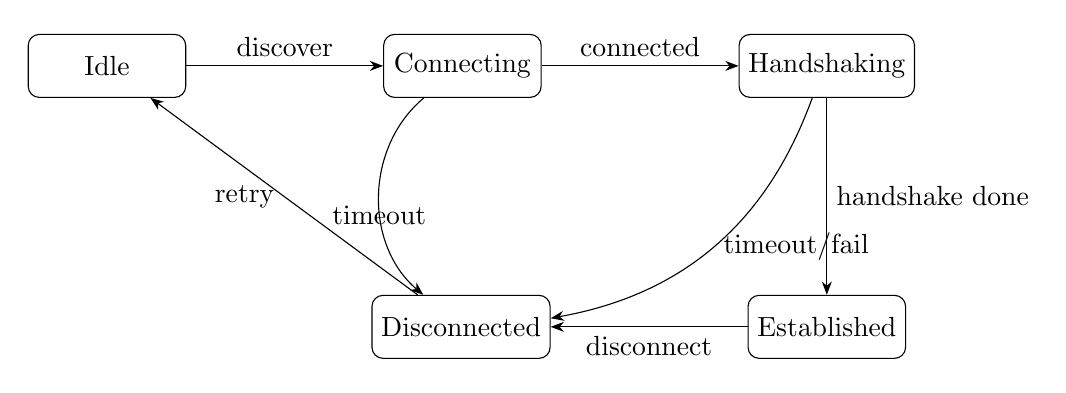
\begin{tikzpicture}[
    ->,
    >=Stealth,
    node distance=2.5cm,
    state/.style={rectangle, rounded corners, draw, minimum width=2cm, minimum height=0.8cm},
    every edge/.style={draw, ->, >=Stealth}
]
    \node[state] (idle) {Idle};
    \node[state, right=of idle] (connecting) {Connecting};
    \node[state, right=of connecting] (handshaking) {Handshaking};
    \node[state, below=of handshaking] (established) {Established};
    \node[state, left=of established] (disconnected) {Disconnected};

    \path (idle) edge node[above] {discover} (connecting);
    \path (connecting) edge node[above] {connected} (handshaking);
    \path (handshaking) edge node[right] {handshake done} (established);
    \path (established) edge node[below] {disconnect} (disconnected);
    \path (disconnected) edge node[left] {retry} (idle);
    \path (connecting) edge[bend right=50] node[below] {timeout} (disconnected);
    \path (handshaking) edge[bend left=30] node[right] {timeout/fail} (disconnected);
\end{tikzpicture}
\end{center}

\mypara{States}
\begin{itemize}
  \item \textbf{Idle:} No connection; scanning or advertising
  \item \textbf{Connecting:} BLE GATT connection in progress
  \item \textbf{Handshaking:} Noise XX handshake in progress
  \item \textbf{Established:} Secure session active; can exchange messages
  \item \textbf{Disconnected:} Connection lost; may retry
\end{itemize}

\subsection{Noise Handshake Flow}

The XX handshake requires 3 messages. The \emph{initiator} is whoever initiated the BLE connection.

\begin{enumerate}
  \item \textbf{Initiator $\to$ Responder:} \texttt{noiseHandshakeInit} (0x10)
    \begin{itemize}
      \item Contains: Initiator's ephemeral public key
    \end{itemize}
  \item \textbf{Responder $\to$ Initiator:} \texttt{noiseHandshakeResp} (0x11)
    \begin{itemize}
      \item Contains: Responder's ephemeral public key + encrypted static key
    \end{itemize}
  \item \textbf{Initiator $\to$ Responder:} \texttt{noiseHandshakeFinal} (0x12)
    \begin{itemize}
      \item Contains: Initiator's encrypted static key
    \end{itemize}
\end{enumerate}

After message 3, both parties derive symmetric transport keys. All subsequent packets are encrypted.

\mypara{Handshake Timeout}
If any handshake message is not received within \texttt{HANDSHAKE\_TIMEOUT} (10 seconds), the connection is aborted.

\subsection{Friendship Request Flow}

\begin{center}
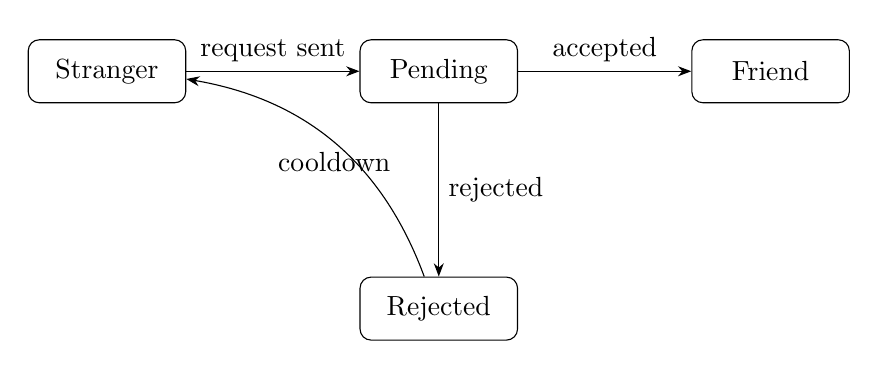
\begin{tikzpicture}[
    ->,
    >=Stealth,
    node distance=2.2cm,
    state/.style={rectangle, rounded corners, draw, minimum width=2cm, minimum height=0.8cm},
]
    \node[state] (none) {Stranger};
    \node[state, right=of none] (pending) {Pending};
    \node[state, right=of pending] (friend) {Friend};
    \node[state, below=of pending] (rejected) {Rejected};

    \path (none) edge node[above] {request sent} (pending);
    \path (pending) edge node[above] {accepted} (friend);
    \path (pending) edge node[right] {rejected} (rejected);
    \path (rejected) edge[bend right=30] node[below] {cooldown} (none);
\end{tikzpicture}
\end{center}

\mypara{Flow}
\begin{enumerate}
  \item $P$ sends \texttt{friendRequest} to $Q$
  \item $Q$ verifies signature on request
  \item $Q$ prompts user (or auto-accepts based on policy)
  \item $Q$ sends \texttt{friendAccept} or \texttt{friendReject}
  \item If accepted, both store each other's keys; if rejected, $P$ waits \texttt{FRIEND\_COOLDOWN} before retrying
\end{enumerate}

%%%%%%%%%%%%%%%%%%%%%%%%%%%%%%%%%%%%%%%%%%%%%%%%%%%%%%%%%%%%%%%%%%%%%%%%%%%%%%%
\section{Data Structures}
\label{sec:datastructures}
%%%%%%%%%%%%%%%%%%%%%%%%%%%%%%%%%%%%%%%%%%%%%%%%%%%%%%%%%%%%%%%%%%%%%%%%%%%%%%%

\subsection{Local Social Graph}

Each device maintains a local database with the following tables:

\mypara{Friends Table}
\begin{tabular}{|l|l|l|}
\hline
\textbf{Field} & \textbf{Type} & \textbf{Description} \\
\hline
peer\_id & BLOB(8) & Primary key (truncated fingerprint) \\
noise\_pk & BLOB(32) & Curve25519 public key \\
sign\_pk & BLOB(32) & Ed25519 public key \\
display\_name & TEXT & User's display name \\
added\_at & INTEGER & Unix timestamp \\
last\_seen & INTEGER & Unix timestamp of last contact \\
is\_verified & BOOLEAN & Out-of-band verification done \\
\hline
\end{tabular}

\mypara{Friends-of-Friends Table}
\begin{tabular}{|l|l|l|}
\hline
\textbf{Field} & \textbf{Type} & \textbf{Description} \\
\hline
peer\_id & BLOB(8) & PeerID of friend-of-friend \\
via\_friend & BLOB(8) & PeerID of mutual friend \\
noise\_pk & BLOB(32) & Public key (if known) \\
display\_name & TEXT & Name (if known) \\
\hline
\end{tabular}

\mypara{Messages Table}
\begin{tabular}{|l|l|l|}
\hline
\textbf{Field} & \textbf{Type} & \textbf{Description} \\
\hline
message\_id & BLOB(16) & UUID \\
sender\_id & BLOB(8) & Sender's PeerID \\
recipient\_id & BLOB(8) & Recipient's PeerID (null for broadcast) \\
content & TEXT & Message content \\
timestamp & INTEGER & Creation time \\
status & INTEGER & 0=pending, 1=sent, 2=delivered, 3=read \\
retry\_count & INTEGER & Number of send attempts \\
\hline
\end{tabular}

\subsection{Bloom Filter for Deduplication}

Each device maintains a Bloom filter to track recently seen packet IDs.

\mypara{Parameters}
\begin{itemize}
  \item Size ($m$): 8192 bits (1 KB)
  \item Hash functions ($k$): 7
  \item Expected elements ($n$): 1000 packets
  \item False positive rate: $\approx 0.8\%$
\end{itemize}

\mypara{Hash Functions}
Use double hashing with MurmurHash3:
\[
h_i(x) = (h_1(x) + i \cdot h_2(x)) \mod m
\]
where $h_1$ and $h_2$ are derived from MurmurHash3 of the packet's (SenderID, Timestamp) tuple.

\mypara{Filter Rotation}
The filter is cleared every \texttt{BLOOM\_ROTATION\_INTERVAL} (5 minutes) to prevent saturation.

\subsection{Friend List Bloom Filter (Level 4)}

For sharing friend lists at Level 4, a separate Bloom filter is used.

\mypara{Parameters}
\begin{itemize}
  \item Size ($m$): 2048 bits (256 bytes)
  \item Hash functions ($k$): 5
  \item Expected elements ($n$): 150 friends
  \item False positive rate: $\approx 1\%$
\end{itemize}

\mypara{Contents}
The filter contains the 8-byte PeerID of each friend.

\mypara{Matching}
When $P$ receives $Q$'s friend list filter:
\begin{enumerate}
  \item For each of $P$'s friends $R$, check if $R$'s PeerID is in $Q$'s filter
  \item If match found, $R$ is likely a mutual friend (subject to false positive rate)
  \item $P$ can then request introduction via $R$
\end{enumerate}

%%%%%%%%%%%%%%%%%%%%%%%%%%%%%%%%%%%%%%%%%%%%%%%%%%%%%%%%%%%%%%%%%%%%%%%%%%%%%%%
\section{Routing and Relay}
%%%%%%%%%%%%%%%%%%%%%%%%%%%%%%%%%%%%%%%%%%%%%%%%%%%%%%%%%%%%%%%%%%%%%%%%%%%%%%%

\subsection{TTL-Based Flooding}

Messages propagate via flooding with TTL limiting:
\begin{enumerate}
  \item Sender sets initial TTL (default: 7)
  \item Each relay decrements TTL
  \item Packet dropped when TTL reaches 0
  \item Bloom filter tracks seen packet IDs to prevent loops
\end{enumerate}

\subsection{Relay Policy by Privacy Level}

\begin{itemize}
  \item \textbf{Level 1:} Does not relay
  \item \textbf{Levels 2--4:} Relay messages for friends and friends-of-friends
\end{itemize}

A user relays a message if:
\begin{enumerate}
  \item The sender is a friend, OR
  \item The sender is a friend-of-friend (known via Level 4 friend list sharing), OR
  \item The recipient is a friend or friend-of-friend
\end{enumerate}

\subsection{Delivery Acknowledgments}

When a private message reaches its destination:
\begin{enumerate}
  \item Recipient sends \texttt{deliveryAck} back to sender
  \item If no ack received within timeout, sender retries
  \item Exponential backoff: 2s, 4s, 8s, 16s (max 4 retries)
\end{enumerate}

\subsection{Store and Forward}

When a message cannot be delivered immediately:
\begin{enumerate}
  \item Message is stored in local queue with status ``pending''
  \item When recipient (or relay path to recipient) becomes available, message is sent
  \item Messages older than \texttt{MESSAGE\_EXPIRY} (24 hours) are discarded
\end{enumerate}

%%%%%%%%%%%%%%%%%%%%%%%%%%%%%%%%%%%%%%%%%%%%%%%%%%%%%%%%%%%%%%%%%%%%%%%%%%%%%%%
\section{Timeouts and Limits}
\label{sec:timeouts}
%%%%%%%%%%%%%%%%%%%%%%%%%%%%%%%%%%%%%%%%%%%%%%%%%%%%%%%%%%%%%%%%%%%%%%%%%%%%%%%

\begin{table}[H]
\centering
\begin{tabular}{|l|l|l|}
\hline
\textbf{Parameter} & \textbf{Value} & \textbf{Description} \\
\hline
\texttt{CONNECTION\_TIMEOUT} & 10 s & BLE connection establishment \\
\texttt{HANDSHAKE\_TIMEOUT} & 10 s & Noise handshake completion \\
\texttt{IDLE\_TIMEOUT} & 60 s & Disconnect idle connections \\
\texttt{FRAGMENT\_TIMEOUT} & 30 s & Incomplete fragment reassembly \\
\texttt{RETRY\_INITIAL} & 2 s & First retry delay \\
\texttt{RETRY\_MAX} & 16 s & Maximum retry delay \\
\texttt{RETRY\_COUNT} & 4 & Maximum retry attempts \\
\texttt{FRIEND\_COOLDOWN} & 300 s & Wait after friend rejection \\
\texttt{MESSAGE\_EXPIRY} & 86400 s & Store-and-forward max age \\
\texttt{BLOOM\_ROTATION} & 300 s & Dedup filter rotation interval \\
\hline
\end{tabular}
\caption{Protocol timeouts}
\label{tab:timeouts}
\end{table}

\begin{table}[H]
\centering
\begin{tabular}{|l|l|l|}
\hline
\textbf{Parameter} & \textbf{Value} & \textbf{Description} \\
\hline
\texttt{MAX\_MESSAGE\_SIZE} & 65535 bytes & Maximum message payload \\
\texttt{MAX\_DISPLAY\_NAME} & 63 bytes & Maximum name length \\
\texttt{MAX\_FRIENDS} & 1000 & Maximum friends list size \\
\texttt{MAX\_PENDING\_MESSAGES} & 100 & Store-and-forward queue size \\
\texttt{MAX\_FRAGMENTS} & 255 & Maximum fragments per message \\
\texttt{DEFAULT\_TTL} & 7 & Initial TTL for flooding \\
\texttt{BLE\_MTU} & 512 bytes & Assumed BLE MTU \\
\texttt{RSSI\_THRESHOLD} & -50 dBm & Proximity for stranger friending \\
\hline
\end{tabular}
\caption{Protocol limits}
\label{tab:limits}
\end{table}

%%%%%%%%%%%%%%%%%%%%%%%%%%%%%%%%%%%%%%%%%%%%%%%%%%%%%%%%%%%%%%%%%%%%%%%%%%%%%%%
\section{Friendship Establishment}
%%%%%%%%%%%%%%%%%%%%%%%%%%%%%%%%%%%%%%%%%%%%%%%%%%%%%%%%%%%%%%%%%%%%%%%%%%%%%%%

$P$ and $Q$ can become friends in three ways:

\subsection{Proximity Handshake (Level 3+)}

\begin{enumerate}
  \item $P$ and $Q$ discover each other via BLE scanning
  \item If RSSI $\ge$ \texttt{RSSI\_THRESHOLD} (close proximity), prompt user
  \item $P$ sends \texttt{friendRequest} with signed PK
  \item $Q$ accepts or rejects
  \item On accept, both store each other's PK in their friend list
\end{enumerate}

\subsection{Introduction (Level 4)}

\begin{enumerate}
  \item $P$ knows $R$; $Q$ knows $R$; $P$ and $Q$ don't know each other
  \item $P$ receives $Q$'s friend list Bloom filter and detects $R$ as mutual friend
  \item $P$ asks $R$ to introduce them to $Q$
  \item $R$ sends \texttt{introduction} packet to $Q$ containing $P$'s PK
  \item $Q$ decides whether to accept $P$ as a friend
\end{enumerate}

\subsection{Cold Call (Out-of-Band)}

\begin{enumerate}
  \item $P$ obtains $Q$'s PK via out-of-band channel (QR code, website, etc.)
  \item $P$ adds $Q$ as a friend locally
  \item When $P$ and $Q$ are in BLE range, $P$ can connect to $Q$'s UUID
  \item $P$ sends \texttt{friendRequest}; $Q$ decides to accept or reject
\end{enumerate}

%%%%%%%%%%%%%%%%%%%%%%%%%%%%%%%%%%%%%%%%%%%%%%%%%%%%%%%%%%%%%%%%%%%%%%%%%%%%%%%
\section{Security Considerations}
%%%%%%%%%%%%%%%%%%%%%%%%%%%%%%%%%%%%%%%%%%%%%%%%%%%%%%%%%%%%%%%%%%%%%%%%%%%%%%%

\begin{itemize}
  \item \textbf{Replay attacks:} Noise transport messages include incrementing nonces; sliding window replay protection
  \item \textbf{Denial of service:} Rate limiting on handshake attempts per peer
  \item \textbf{Man-in-the-middle:} XX pattern authenticates both parties; users should verify fingerprints out-of-band for high-security contacts
  \item \textbf{Traffic analysis:} Fixed-size padding obscures message lengths
  \item \textbf{Fingerprinting:} Per-user Service UUIDs are a tradeoff; users accept identifiability at Levels 2+ in exchange for friend discovery
\end{itemize}

%%%%%%%%%%%%%%%%%%%%%%%%%%%%%%%%%%%%%%%%%%%%%%%%%%%%%%%%%%%%%%%%%%%%%%%%%%%%%%%
\section{Conclusion}
%%%%%%%%%%%%%%%%%%%%%%%%%%%%%%%%%%%%%%%%%%%%%%%%%%%%%%%%%%%%%%%%%%%%%%%%%%%%%%%

This protocol enables resilient, decentralized communication over BLE with customizable privacy levels. By deriving Service UUIDs from public keys, friends can discover each other without central infrastructure. The four privacy levels allow users to balance discoverability against anonymity according to their preferences.

\bibliographystyle{ACM-Reference-Format}
\begin{thebibliography}{1}
\bibitem{bitchat}
BitChat Protocol Whitepaper, Version 1.1, July 2025.
\url{https://github.com/permissionlesstech/bitchat}
\end{thebibliography}

\end{document}
